% Options for packages loaded elsewhere
\PassOptionsToPackage{unicode}{hyperref}
\PassOptionsToPackage{hyphens}{url}
\PassOptionsToPackage{dvipsnames,svgnames,x11names}{xcolor}
%
\documentclass[
  11pt,
  letterpaper,
  DIV=11,
  numbers=noendperiod]{scrreprt}

\usepackage{amsmath,amssymb}
\usepackage{lmodern}
\usepackage{iftex}
\ifPDFTeX
  \usepackage[T1]{fontenc}
  \usepackage[utf8]{inputenc}
  \usepackage{textcomp} % provide euro and other symbols
\else % if luatex or xetex
  \usepackage{unicode-math}
  \defaultfontfeatures{Scale=MatchLowercase}
  \defaultfontfeatures[\rmfamily]{Ligatures=TeX,Scale=1}
\fi
% Use upquote if available, for straight quotes in verbatim environments
\IfFileExists{upquote.sty}{\usepackage{upquote}}{}
\IfFileExists{microtype.sty}{% use microtype if available
  \usepackage[]{microtype}
  \UseMicrotypeSet[protrusion]{basicmath} % disable protrusion for tt fonts
}{}
\makeatletter
\@ifundefined{KOMAClassName}{% if non-KOMA class
  \IfFileExists{parskip.sty}{%
    \usepackage{parskip}
  }{% else
    \setlength{\parindent}{0pt}
    \setlength{\parskip}{6pt plus 2pt minus 1pt}}
}{% if KOMA class
  \KOMAoptions{parskip=half}}
\makeatother
\usepackage{xcolor}
\usepackage[margin=1in]{geometry}
\setlength{\emergencystretch}{3em} % prevent overfull lines
\setcounter{secnumdepth}{5}
% Make \paragraph and \subparagraph free-standing
\ifx\paragraph\undefined\else
  \let\oldparagraph\paragraph
  \renewcommand{\paragraph}[1]{\oldparagraph{#1}\mbox{}}
\fi
\ifx\subparagraph\undefined\else
  \let\oldsubparagraph\subparagraph
  \renewcommand{\subparagraph}[1]{\oldsubparagraph{#1}\mbox{}}
\fi


\providecommand{\tightlist}{%
  \setlength{\itemsep}{0pt}\setlength{\parskip}{0pt}}\usepackage{longtable,booktabs,array}
\usepackage{calc} % for calculating minipage widths
% Correct order of tables after \paragraph or \subparagraph
\usepackage{etoolbox}
\makeatletter
\patchcmd\longtable{\par}{\if@noskipsec\mbox{}\fi\par}{}{}
\makeatother
% Allow footnotes in longtable head/foot
\IfFileExists{footnotehyper.sty}{\usepackage{footnotehyper}}{\usepackage{footnote}}
\makesavenoteenv{longtable}
\usepackage{graphicx}
\makeatletter
\def\maxwidth{\ifdim\Gin@nat@width>\linewidth\linewidth\else\Gin@nat@width\fi}
\def\maxheight{\ifdim\Gin@nat@height>\textheight\textheight\else\Gin@nat@height\fi}
\makeatother
% Scale images if necessary, so that they will not overflow the page
% margins by default, and it is still possible to overwrite the defaults
% using explicit options in \includegraphics[width, height, ...]{}
\setkeys{Gin}{width=\maxwidth,height=\maxheight,keepaspectratio}
% Set default figure placement to htbp
\makeatletter
\def\fps@figure{htbp}
\makeatother
\newlength{\cslhangindent}
\setlength{\cslhangindent}{1.5em}
\newlength{\csllabelwidth}
\setlength{\csllabelwidth}{3em}
\newlength{\cslentryspacingunit} % times entry-spacing
\setlength{\cslentryspacingunit}{\parskip}
\newenvironment{CSLReferences}[2] % #1 hanging-ident, #2 entry spacing
 {% don't indent paragraphs
  \setlength{\parindent}{0pt}
  % turn on hanging indent if param 1 is 1
  \ifodd #1
  \let\oldpar\par
  \def\par{\hangindent=\cslhangindent\oldpar}
  \fi
  % set entry spacing
  \setlength{\parskip}{#2\cslentryspacingunit}
 }%
 {}
\usepackage{calc}
\newcommand{\CSLBlock}[1]{#1\hfill\break}
\newcommand{\CSLLeftMargin}[1]{\parbox[t]{\csllabelwidth}{#1}}
\newcommand{\CSLRightInline}[1]{\parbox[t]{\linewidth - \csllabelwidth}{#1}\break}
\newcommand{\CSLIndent}[1]{\hspace{\cslhangindent}#1}

\KOMAoption{captions}{tableheading,figureheading}
\makeatletter
\@ifpackageloaded{tcolorbox}{}{\usepackage[many]{tcolorbox}}
\@ifpackageloaded{fontawesome5}{}{\usepackage{fontawesome5}}
\definecolor{quarto-callout-color}{HTML}{909090}
\definecolor{quarto-callout-note-color}{HTML}{0758E5}
\definecolor{quarto-callout-important-color}{HTML}{CC1914}
\definecolor{quarto-callout-warning-color}{HTML}{EB9113}
\definecolor{quarto-callout-tip-color}{HTML}{00A047}
\definecolor{quarto-callout-caution-color}{HTML}{FC5300}
\definecolor{quarto-callout-color-frame}{HTML}{acacac}
\definecolor{quarto-callout-note-color-frame}{HTML}{4582ec}
\definecolor{quarto-callout-important-color-frame}{HTML}{d9534f}
\definecolor{quarto-callout-warning-color-frame}{HTML}{f0ad4e}
\definecolor{quarto-callout-tip-color-frame}{HTML}{02b875}
\definecolor{quarto-callout-caution-color-frame}{HTML}{fd7e14}
\makeatother
\makeatletter
\makeatother
\makeatletter
\@ifpackageloaded{bookmark}{}{\usepackage{bookmark}}
\makeatother
\makeatletter
\@ifpackageloaded{caption}{}{\usepackage{caption}}
\AtBeginDocument{%
\ifdefined\contentsname
  \renewcommand*\contentsname{Table of contents}
\else
  \newcommand\contentsname{Table of contents}
\fi
\ifdefined\listfigurename
  \renewcommand*\listfigurename{List of Figures}
\else
  \newcommand\listfigurename{List of Figures}
\fi
\ifdefined\listtablename
  \renewcommand*\listtablename{List of Tables}
\else
  \newcommand\listtablename{List of Tables}
\fi
\ifdefined\figurename
  \renewcommand*\figurename{Figure}
\else
  \newcommand\figurename{Figure}
\fi
\ifdefined\tablename
  \renewcommand*\tablename{Table}
\else
  \newcommand\tablename{Table}
\fi
}
\@ifpackageloaded{float}{}{\usepackage{float}}
\floatstyle{ruled}
\@ifundefined{c@chapter}{\newfloat{codelisting}{h}{lop}}{\newfloat{codelisting}{h}{lop}[chapter]}
\floatname{codelisting}{Listing}
\newcommand*\listoflistings{\listof{codelisting}{List of Listings}}
\makeatother
\makeatletter
\@ifpackageloaded{caption}{}{\usepackage{caption}}
\@ifpackageloaded{subcaption}{}{\usepackage{subcaption}}
\makeatother
\makeatletter
\@ifpackageloaded{tcolorbox}{}{\usepackage[many]{tcolorbox}}
\makeatother
\makeatletter
\@ifundefined{shadecolor}{\definecolor{shadecolor}{rgb}{.97, .97, .97}}
\makeatother
\makeatletter
\makeatother
\ifLuaTeX
  \usepackage{selnolig}  % disable illegal ligatures
\fi
\IfFileExists{bookmark.sty}{\usepackage{bookmark}}{\usepackage{hyperref}}
\IfFileExists{xurl.sty}{\usepackage{xurl}}{} % add URL line breaks if available
\urlstyle{same} % disable monospaced font for URLs
\hypersetup{
  pdftitle={Comparing LLM and human peer reviews and ratings of social science research using data from Unjournal.org evaluations},
  pdfauthor={David Reinstein; Valentin Klotzbücher},
  colorlinks=true,
  linkcolor={blue},
  filecolor={Maroon},
  citecolor={Blue},
  urlcolor={Blue},
  pdfcreator={LaTeX via pandoc}}

\title{Comparing LLM and human peer reviews and ratings of social
science research using data from Unjournal.org evaluations}
\author{David Reinstein \and Valentin Klotzbücher}
\date{2025-09-02T17:54:46+01:00}

\begin{document}
\maketitle
\begin{abstract}
We will build and refine LLM tools to generate peer-reviews and ratings
of impactful research, and compare these with human experts' work
(esp.~from Unjournal.org): to benchmark performance, understand AI's
research taste, and develop tools to improve research evaluation and
dissemination.
\end{abstract}
\ifdefined\Shaded\renewenvironment{Shaded}{\begin{tcolorbox}[enhanced, sharp corners, breakable, interior hidden, borderline west={3pt}{0pt}{shadecolor}, boxrule=0pt, frame hidden]}{\end{tcolorbox}}\fi

\renewcommand*\contentsname{Table of contents}
{
\hypersetup{linkcolor=}
\setcounter{tocdepth}{2}
\tableofcontents
}
\bookmarksetup{startatroot}

\hypertarget{project-overview}{%
\chapter{Project Overview}\label{project-overview}}

\begin{tcolorbox}[enhanced jigsaw, opacitybacktitle=0.6, left=2mm, opacityback=0, coltitle=black, titlerule=0mm, colback=white, title=\textcolor{quarto-callout-warning-color}{\faExclamationTriangle}\hspace{0.5em}{Warning}, bottomrule=.15mm, colbacktitle=quarto-callout-warning-color!10!white, bottomtitle=1mm, toptitle=1mm, breakable, arc=.35mm, rightrule=.15mm, toprule=.15mm, leftrule=.75mm, colframe=quarto-callout-warning-color-frame]
Work in progress. Pages, metrics, and comparisons are under active
development. Expect rough edges and frequent updates.
\end{tcolorbox}

\hypertarget{motivation-and-questions}{%
\section{Motivation and questions}\label{motivation-and-questions}}

Is AI good at peer-reviewing? Does it offer useful and valid feedback?
Can it predict how human experts will rate research across a range of
categories? How can it help academics do this ``thankless'' task better?
Is it particularly good at spotting errors? Are there specific
categories, e.g.~spotting math errors or judging real-world relevance,
where it does surprisingly well or poorly? How does its ``research
taste'' compare to humans?

If AI research-evaluation works it could free up a lot of scientific
resources -- perhaps \$1.5 billion/year in the US alone (Aczel, Szaszi,
and Holcombe (\protect\hyperlink{ref-aczel2021billion}{2021}))) -- and
offer more continual and detailed review, helping improve research. It
could also help characterize methodological strengths/weaknesses across
papers, aiding training and research direction-setting. Furthermore, a
key promise of AI is to directly improve science and research.
Understanding how AI engages with research evaluations may provide a
window into its values, abilities, and limitations.

In this project, we are testing the capabilities of current large
language models (LLMs), illustrating whether they can generate research
paper evaluations comparable to expert human reviews. The Unjournal
systematically prioritizes `impactful' research and pays for
high-quality human evaluations, structured quantified ratings, claim
identification and assessment, and predictions. In this project, we use
an AI (OpenAI's \texttt{GPT-5} model for now) to review social science
research papers under the same criteria used by human reviewers for The
Unjournal.

Each paper is assessed on specific dimensions -- for example, the
strength of its evidence, rigor of methods, clarity of communication,
openness/reproducibility, relevance to global priorities, and overall
quality. The LLM will provide quantitative scores (with uncertainty
intervals) on these criteria and produce a written evaluation

Our initial dataset will include research papers that have existing
human evaluations. For each paper, the AI will generate: (1) numeric
ratings on the defined criteria, (2) identification of the paper's key
claims, and (3) a detailed review discussing the paper's contributions
and weaknesses. We will then compare the AI-generated evaluations to the
published human evaluations.

Next, we will focus on papers currently under evaluation, ie where no
human evaluation exists yet and we can rule out any contamination.

\hypertarget{related-work}{%
\section{Related work}\label{related-work}}

Luo et al. (\protect\hyperlink{ref-Luo2025}{2025}) survey LLM roles from
idea generation to peer review, including experiment planning and
automated scientific writing. They highlight opportunities
(productivity, coverage of long documents) alongside governance needs
(provenance, detection of LLM-generated content, standardizing tooling)
and call for reliable evaluation frameworks.

Eger et al. (\protect\hyperlink{ref-eger2025}{2025}) provide a broad
review of LLMs in science and a focused discussion of AI‑assisted peer
review. They emphasize: (i) peer‑review data is scarce and concentrated
in CS/OpenReview venues; (ii) targeted assistance that preserves human
autonomy is preferable to end‑to‑end reviewing; and (iii) ethics and
governance (bias, provenance, detection of AI‑generated text) are
first‑class constraints.

Zhang and Abernethy (\protect\hyperlink{ref-Zhang2025}{2025}) propose
deploying LLMs as quality checkers to surface critical problems instead
of generating full narrative reviews. Using papers from WITHDRARXIV and
an automatic evaluation framework that leverages ``LLM-as-judge,'' they
find the best performance from top reasoning models but still recommend
human oversight.

\bookmarksetup{startatroot}

\hypertarget{numerical-ratings-llm-work}{%
\chapter{Numerical ratings (LLM
work)}\label{numerical-ratings-llm-work}}

We evaluate each paper along the following dimensions: \textbf{claims \&
evidence}, \textbf{methods}, \textbf{logic \& communication},
\textbf{open science}, \textbf{global relevance}, and an
\textbf{overall} assessment. Ratings are interpreted as percentiles
relative to serious recent work in the same area. For each metric the
model returns a midpoint and a 90\% credible interval to communicate
uncertainty.

We iterate over \texttt{papers/*.pdf}, collect raw results and write a
long CSV to \texttt{results/metrics\_long.csv}.

\begin{center}\rule{0.5\linewidth}{0.5pt}\end{center}

\bookmarksetup{startatroot}

\hypertarget{llm-vs.-human-ratings}{%
\chapter{LLM vs.~Human Ratings}\label{llm-vs.-human-ratings}}

This page compares the LLM‑generated ratings (\texttt{gpt-5}) from
the\protect\hyperlink{numerical-ratings-llm-work}{(previous section}
with human evaluations across
\href{https://globalimpact.gitbook.io/the-unjournal-project-and-communication-space/policies-projects-evaluation-workflow/evaluation/guidelines-for-evaluators\#undefined-1}{the
Unjournal's criteria}. We (i) harmonize the two sources to a common set
of metrics and paper IDs, (ii) compute paired scores per \emph{(paper,
metric)}, and (iii) summarize agreement using distributional views and
reliability statistics.

\hypertarget{data-harmonization}{%
\section{Data \& Harmonization}\label{data-harmonization}}

\begin{itemize}
\tightlist
\item
  Sources. LLM ratings come from \texttt{results/metrics\_long.csv}
  (rendered in the previous chapter). Human ratings are imported from
  your hand‑coded spreadsheet and mapped to LLM paper IDs via
  \texttt{UJ\_map.csv}.\\
\item
  Metric alignment. Human criteria are recoded to the LLM schema (e.g.,
  \texttt{claims} → \texttt{claims\_evidence}, \texttt{adv\_knowledge} →
  \texttt{advancing\_knowledge}, etc.). If humans provided both
  \texttt{gp\_relevance} and \texttt{real\_world}, we fold these into
  the single LLM metric \texttt{global\_relevance}.\\
\item
  Uncertainty fields. Where available, we carry lower/upper bounds for
  both LLM and humans; these are used in optional uncertainty checks but
  do not affect the mid‑point comparisons below.
\end{itemize}

\hypertarget{distribution-of-ratings}{%
\section{Distribution of ratings}\label{distribution-of-ratings}}

\begin{figure}

\caption{\label{fig-scatter-ellipses}\textbf{?(caption)}}

\begin{figure}

\caption{LLM vs Human with robust CI ellipses. Horizontal span covers
the union of all human raters' CIs and point ratings; vertical span from
LLM CI. Centers at midpoints. Dropdown selects metric.}

\begin{verbatim}
Unable to display output for mime type(s): text/html
\end{verbatim}

\end{figure}

\begin{figure}

\caption{\textbf{?(caption)}}

\begin{verbatim}
Unable to display output for mime type(s): text/html
\end{verbatim}

\end{figure}

\end{figure}

For each paper (selected metric), the \textbf{ellipse} is centered at
the pair of midpoints \emph{(Human, LLM)}. The \textbf{horizontal
radius} covers the \emph{union} of all human evidence for that paper ---
combining individual raters' point scores and their CIs --- while the
\textbf{vertical radius} reflects the LLM CI. This makes the ellipse
wide enough to contain every human point horizontally (unless a point
lies outside its own stated CI, which is flagged in a diagnostic check).

\begin{figure}

\caption{\label{fig-hist-static}Distributions by metric. Top: Overall
(full width). Bottom: remaining metrics in a 2×3 grid.}

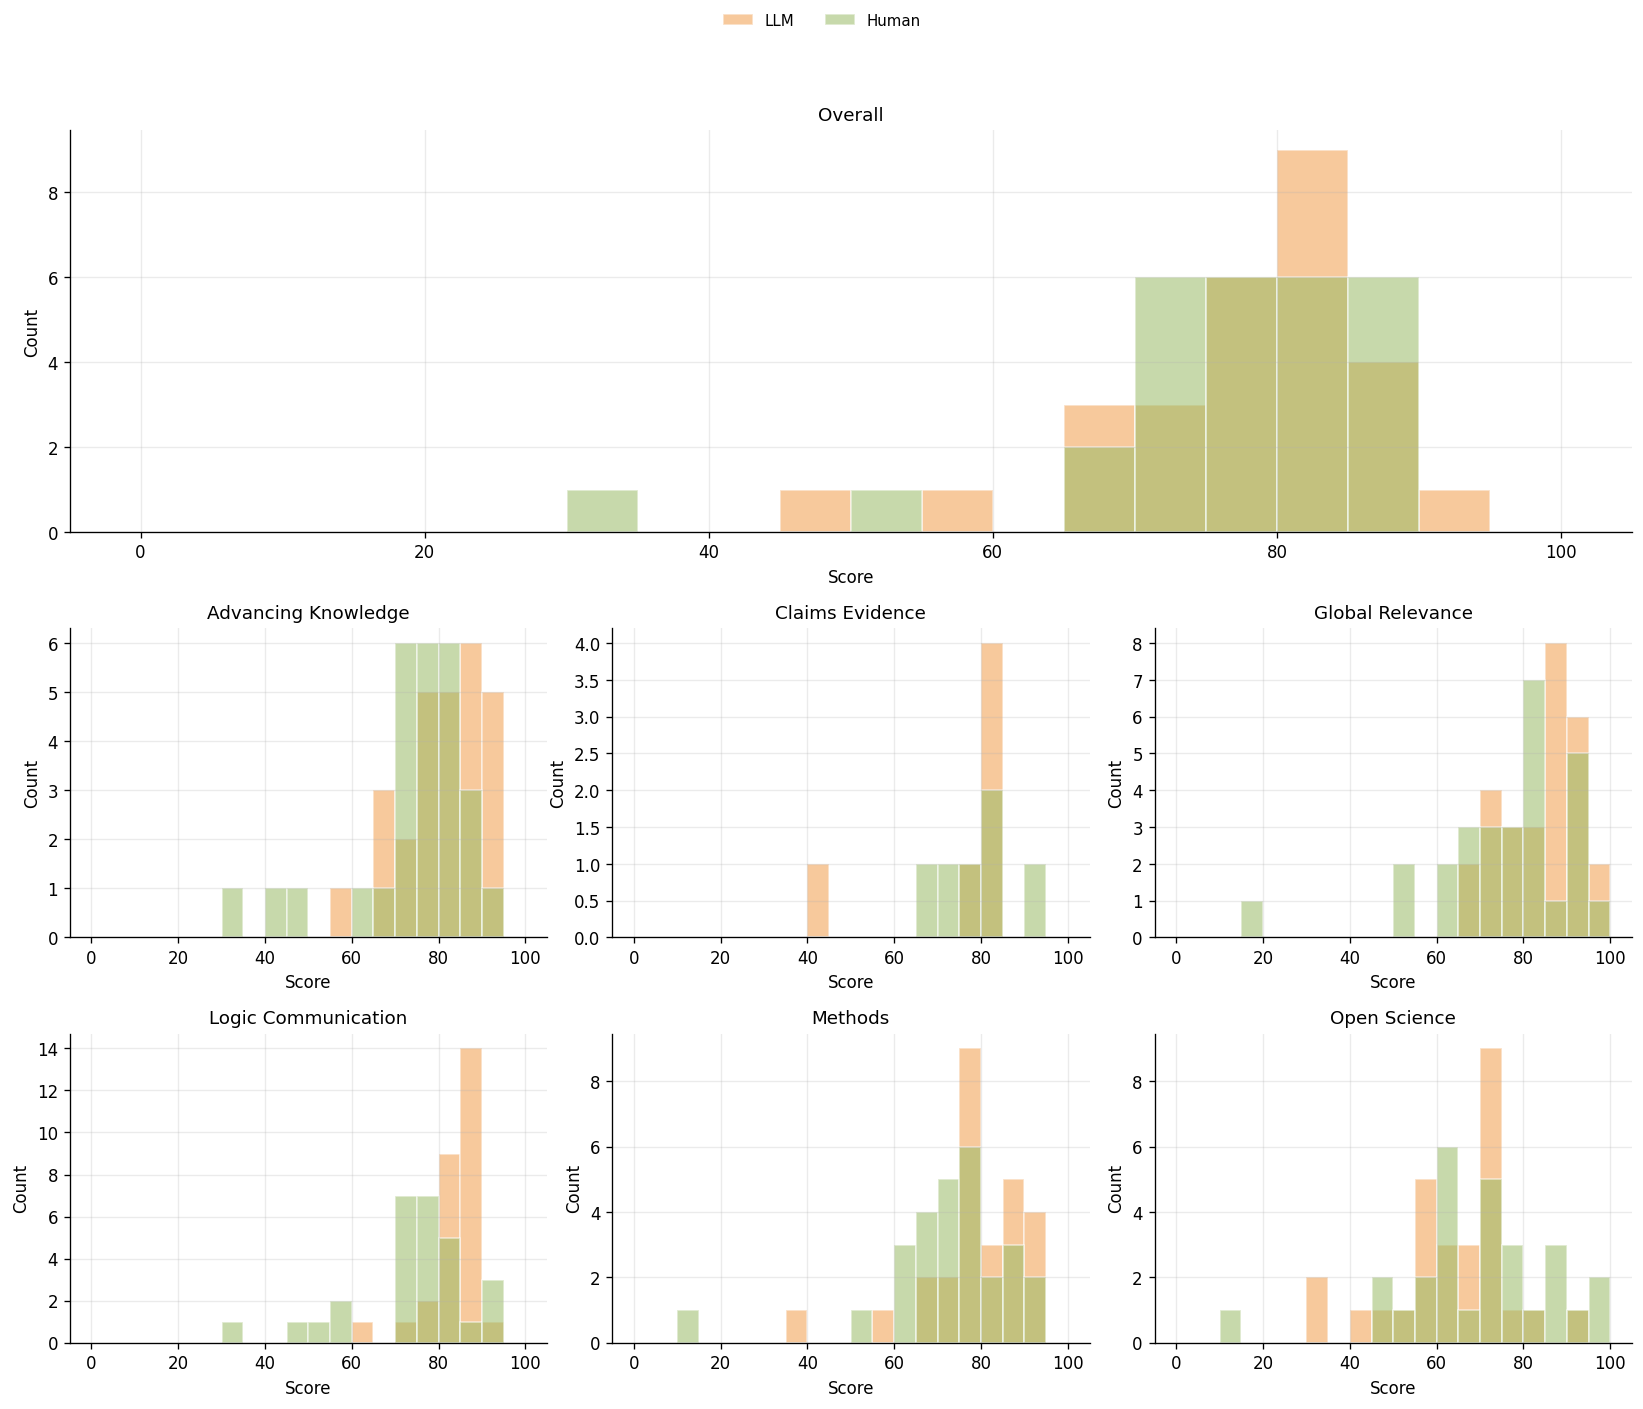
\includegraphics{./compare_ratings_files/figure-pdf/fig-hist-static-output-1.png} \hfill{}

\end{figure}

\hypertarget{differences-by-paper-and-metric}{%
\section{Differences by paper and
metric}\label{differences-by-paper-and-metric}}

For each \emph{(paper, metric)}, we plot LLM − Human difference in
Figure~\ref{fig-heatmap-static}. Green means the LLM is lower than the
human midpoint; orange means higher.

\begin{itemize}
\tightlist
\item
  Vertical stripes (by metric) suggest a metric‑specific bias (LLM
  systematically up/down on that metric).\\
\item
  Horizontal stripes (by paper) flag paper‑specific disagreement (LLM
  consistently above/below for that paper across metrics).\\
\item
  Isolated bright cells highlight individual outliers worth auditing
  qualitatively.
\end{itemize}

\begin{figure}

\caption{\label{fig-heatmap-static}LLM − Human difference by paper ×
metric (robust, centered scale; rows sorted by signed overall
difference).}

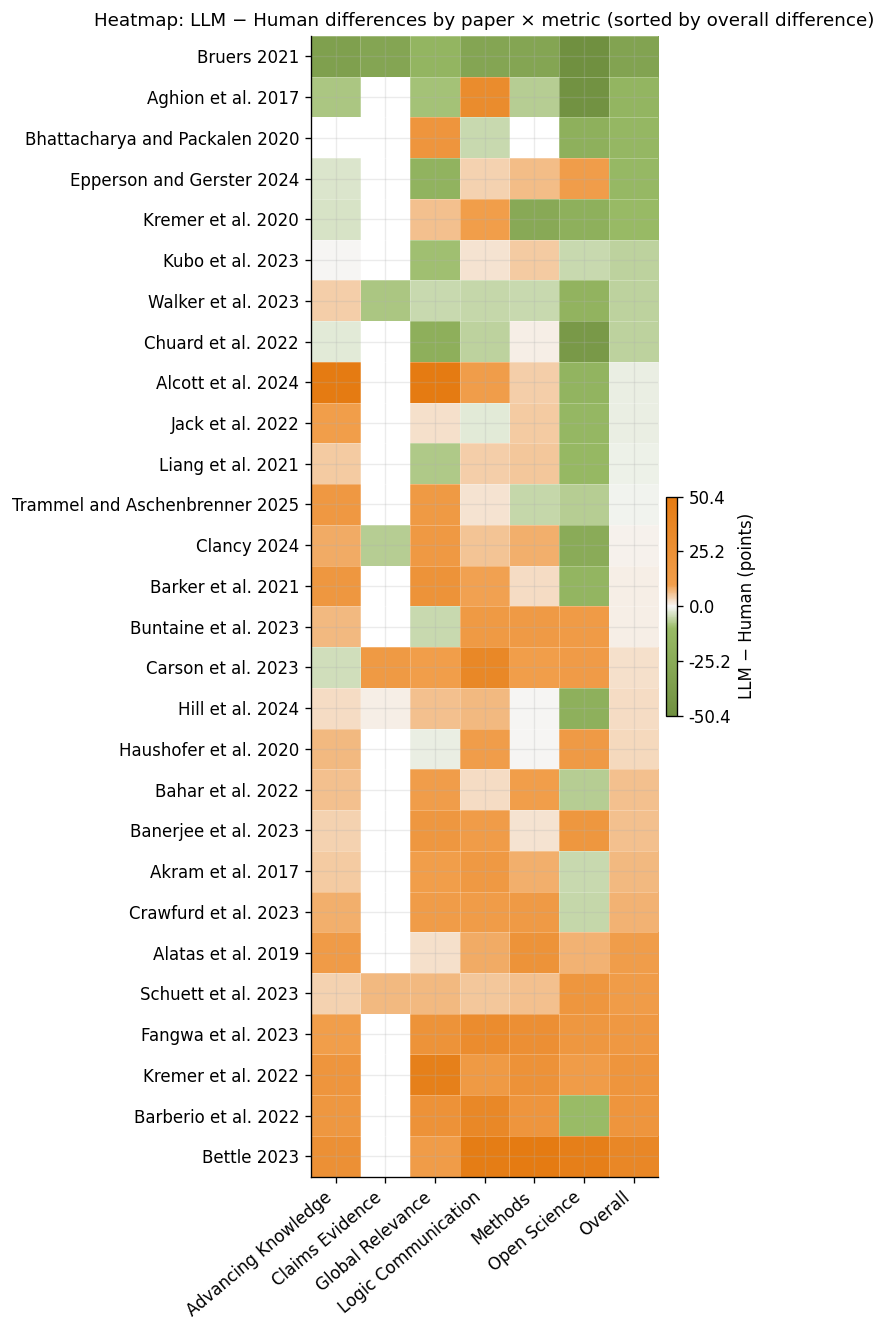
\includegraphics{./compare_ratings_files/figure-pdf/fig-heatmap-static-output-1.png} \hfill{}

\end{figure}

\hypertarget{agreement-metrics}{%
\section{Agreement metrics}\label{agreement-metrics}}

Table~\ref{tbl-agreement} summarizes agreement: Pearson (r) captures
linear alignment of levels; Spearman (ρ) captures rank agreement
(monotonic relationship), robust to scale differences. We report the
mean and median of (LLM − Human) to summarize both average shift and
central tendency of the differences and Cohen's κ (unweighted \&
quadratic). Because scores are continuous, we discretize both LLM and
Human using shared quantile cutpoints (5 bins) and compute the
Unweighted κ (exact category agreement beyond chance) and the
Quadratic‑weighted κ that penalizes larger disagreements more than
smaller ones.

As another indicator of agreement, we check whether each side's credible
interval contain the other's point estimate, Table~\ref{tbl-coverage}
shows the shares across rating categories.

Table~\ref{tbl-calibration} shows ``calibration'' results based on a
simple linear regression; Figure~\ref{fig-uncert-vs-error} plots the
width of human raters CI against the difference in ratings; and
Table~\ref{tbl-outliers} lists the papers with the largest aabsolute
difference between LLM and human raters.

\hypertarget{tbl-agreement}{}
\begin{longtable}[]{@{}lllllllll@{}}
\caption{\label{tbl-agreement}Agreement metrics by metric (Pearson,
Spearman, mean/median bias, κ unweighted/weighted).}\tabularnewline
\toprule()
& metric & n & pearson & spearman & mean\_bias & median\_bias &
kappa\_unwtd & kappa\_quad \\
\midrule()
\endfirsthead
\toprule()
& metric & n & pearson & spearman & mean\_bias & median\_bias &
kappa\_unwtd & kappa\_quad \\
\midrule()
\endhead
0 & advancing\_knowledge & 27 & 0.198 & 0.259 & 7.12 & 6.0 & 0.052 &
0.257 \\
1 & claims\_evidence & 6 & 0.410 & 0.471 & -3.75 & -3.0 & -0.154 &
0.400 \\
2 & global\_relevance & 28 & 0.135 & 0.109 & 8.21 & 8.5 & -0.040 &
0.070 \\
3 & logic\_communication & 28 & 0.001 & 0.130 & 10.01 & 9.0 & -0.029 &
0.041 \\
4 & methods & 27 & 0.309 & 0.403 & 6.60 & 5.5 & 0.148 & 0.288 \\
5 & open\_science & 28 & 0.138 & 0.103 & -6.01 & -7.0 & 0.009 & 0.137 \\
6 & overall & 28 & 0.280 & 0.309 & 1.64 & 1.0 & 0.125 & 0.374 \\
\bottomrule()
\end{longtable}

\hypertarget{tbl-calibration}{}
\begin{longtable}[]{@{}lllllllll@{}}
\caption{\label{tbl-calibration}Calibration of LLM to Human by metric
(Human ≈ intercept + slope·LLM). Includes pre-/post-
MAD.}\tabularnewline
\toprule()
& metric & n & slope & intercept & r2 & MAD\_pre & MAD\_post &
MAD\_delta \\
\midrule()
\endfirsthead
\toprule()
& metric & n & slope & intercept & r2 & MAD\_pre & MAD\_post &
MAD\_delta \\
\midrule()
\endhead
0 & advancing\_knowledge & 27 & 0.284 & 50.232 & 0.039 & 11.216 & 8.812
& 2.404 \\
1 & claims\_evidence & 6 & 0.220 & 61.234 & 0.168 & 11.250 & 5.859 &
5.391 \\
2 & global\_relevance & 28 & 0.255 & 53.573 & 0.018 & 14.589 & 12.000 &
2.589 \\
3 & logic\_communication & 28 & 0.002 & 72.823 & 0.000 & 13.464 & 9.802
& 3.663 \\
4 & methods & 27 & 0.404 & 39.774 & 0.096 & 12.099 & 9.427 & 2.672 \\
5 & open\_science & 28 & 0.174 & 57.509 & 0.019 & 17.976 & 13.346 &
4.631 \\
6 & overall & 28 & 0.357 & 47.941 & 0.078 & 9.149 & 7.837 & 1.312 \\
\bottomrule()
\end{longtable}

\hypertarget{tbl-coverage}{}
\begin{longtable}[]{@{}llllll@{}}
\caption{\label{tbl-coverage}CI coverage: does one interval contain the
other's point estimate?}\tabularnewline
\toprule()
& metric & N & human\_in\_llm & llm\_in\_human & both\_cover \\
\midrule()
\endfirsthead
\toprule()
& metric & N & human\_in\_llm & llm\_in\_human & both\_cover \\
\midrule()
\endhead
0 & advancing\_knowledge & 24 & 0.67 & 0.62 & 0.54 \\
1 & claims\_evidence & 6 & 0.67 & 0.67 & 0.67 \\
2 & global\_relevance & 25 & 0.36 & 0.44 & 0.28 \\
3 & logic\_communication & 25 & 0.36 & 0.60 & 0.36 \\
4 & methods & 24 & 0.62 & 0.54 & 0.50 \\
5 & open\_science & 25 & 0.48 & 0.40 & 0.28 \\
6 & overall & 25 & 0.60 & 0.60 & 0.52 \\
\bottomrule()
\end{longtable}

\begin{figure}

\caption{\label{fig-uncert-vs-error}Human uncertainty (CI width) vs
\textbar LLM − Human\textbar. Spearman correlation reported.}

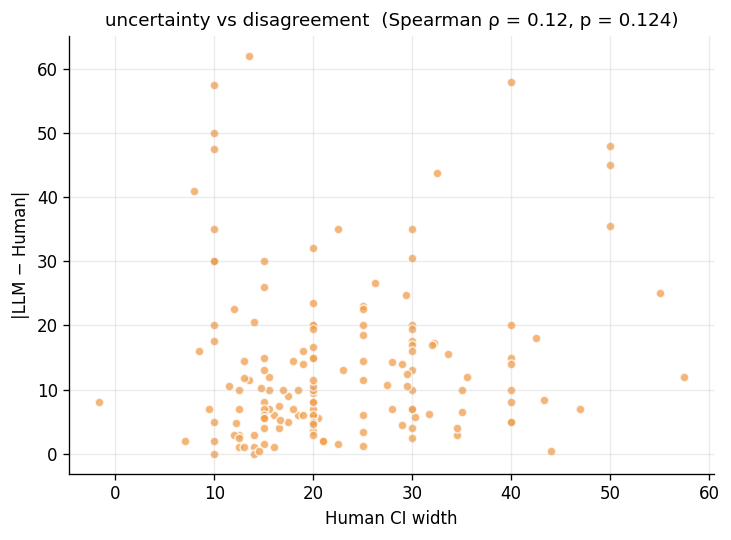
\includegraphics{./compare_ratings_files/figure-pdf/fig-uncert-vs-error-output-1.png} \hfill{}

\end{figure}

\hypertarget{tbl-outliers}{}
\begin{longtable}[]{@{}llllllll@{}}
\caption{\label{tbl-outliers}Top absolute differences (LLM vs Human).
Flags show whether each point lies within the other's
CI.}\tabularnewline
\toprule()
& paper & metric & midpoint\_llm & midpoint\_human & abs\_diff &
human\_in\_llm & llm\_in\_human \\
\midrule()
\endfirsthead
\toprule()
& paper & metric & midpoint\_llm & midpoint\_human & abs\_diff &
human\_in\_llm & llm\_in\_human \\
\midrule()
\endhead
23 & Alcott et al. 2024 & global\_relevance & 78 & 16.00 & 62.00 & False
& False \\
49 & Bettle 2023 & methods & 68 & 10.00 & 58.00 & False & False \\
20 & Alcott et al. 2024 & advancing\_knowledge & 90 & 32.50 & 57.50 &
False & False \\
63 & Bruers 2021 & open\_science & 30 & 80.00 & 50.00 & False & False \\
51 & Bettle 2023 & logic\_communication & 78 & 30.00 & 48.00 & False &
False \\
4 & Aghion et al. 2017 & open\_science & 40 & 87.50 & 47.50 & False &
False \\
52 & Bettle 2023 & open\_science & 55 & 10.00 & 45.00 & False & False \\
139 & Kremer et al. 2022 & global\_relevance & 95 & 51.25 & 43.75 &
False & False \\
82 & Chuard et al. 2022 & open\_science & 55 & 96.00 & 41.00 & False &
False \\
48 & Bettle 2023 & overall & 68 & 32.50 & 35.50 & False & False \\
39 & Barberio et al. 2022 & logic\_communication & 80 & 45.00 & 35.00 &
False & False \\
61 & Bruers 2021 & advancing\_knowledge & 55 & 90.00 & 35.00 & False &
False \\
75 & Carson et al. 2023 & logic\_communication & 85 & 50.00 & 35.00 &
False & False \\
58 & Bruers 2021 & overall & 48 & 80.00 & 32.00 & False & False \\
3 & Aghion et al. 2017 & logic\_communication & 88 & 57.50 & 30.50 &
False & False \\
\bottomrule()
\end{longtable}

\bookmarksetup{startatroot}

\hypertarget{references}{%
\chapter*{References}\label{references}}
\addcontentsline{toc}{chapter}{References}

\hypertarget{refs}{}
\begin{CSLReferences}{1}{0}
\leavevmode\vadjust pre{\hypertarget{ref-aczel2021billion}{}}%
Aczel, Balazs, Barnabas Szaszi, and Alex O Holcombe, {``A billion-dollar
donation: Estimating the cost of researchers' time spent on peer
review,''} \emph{Research integrity and peer review}, 6 (2021), 1--8
(Springer).

\leavevmode\vadjust pre{\hypertarget{ref-eger2025}{}}%
Eger, Steffen, Yong Cao, Jennifer D'Souza, Andreas Geiger, Christian
Greisinger, Stephanie Gross, Yufang Hou, Brigitte Krenn, Anne Lauscher,
Yizhi Li, Chenghua Lin, Nafise Sadat Moosavi, Wei Zhao, and Tristan
Miller, {``\href{https://arxiv.org/abs/2502.05151}{Transforming science
with large language models: A survey on AI-assisted scientific
discovery, experimentation, content generation, and evaluation},''}
\emph{arXiv preprint arXiv:2505.05151}, (2025).

\leavevmode\vadjust pre{\hypertarget{ref-Luo2025}{}}%
Luo, Ziming, Zonglin Yang, Zexin Xu, Wei Yang, and Xinya Du,
{``\href{https://arxiv.org/abs/2501.04306}{LLM4SR: A survey on large
language models for scientific research},''} \emph{arXiv preprint
arXiv:2501.04306}, (2025).

\leavevmode\vadjust pre{\hypertarget{ref-Zhang2025}{}}%
Zhang, Tianmai M, and Neil F Abernethy,
{``\href{https://arxiv.org/abs/2505.23824v2}{Reviewing scientific papers
for critical problems with reasoning LLMs: Baseline approaches and
automatic evaluation},''} \emph{arXiv preprint arXiv:2505.23824},
(2025).

\end{CSLReferences}



\end{document}
